\section*{Appendix A: Intuition on Convergence}

  Unlike convergence of numbers, which is well-defined with respect to some metric or topology, there are many types of convergence of random variables. We must always specify which convergence when talking about them. Remember that a random variable $X$ is just a function from $\Omega$ to $\mathbb{R}$, so we can talk about pointwise convergence. That is, given a sequence of random variables $\{X_n\}$ and some $\omega \in \Omega$, the sequence 
  \begin{equation}
    X_1(\omega), X_2 (\omega), X_3(\omega), \ldots
  \end{equation}
  is simply a sequence of real numbers. If this sequence converges to the real number $X(\omega)$, then $X_n$ converges to $X$ at $\omega$. If this occurs for all $\omega \in \Omega$, then we have sure convergence, and if this happens for an event (a $\mathcal{F}$-measurable subset of $\Omega$) with probability $1$, then we have almost sure convergence. 

  \begin{definition}[Sure Convergence of RVs]
    The sequence of random variables $\{ X_n\}_{n \in \mathbb{N}}$ is said to \textbf{converge pointwise} or \textbf{converge surely} to $X$ if 
    \begin{equation}
      X_n (\omega) \rightarrow X (\omega)
    \end{equation}
    for every $\omega \in \Omega$. That is, we can choose \textit{any} $\omega \in \Omega$, and the realized sequence $X_1 (\omega), X_2 (\omega), \ldots$ will always converge to $X(\omega)$. We can visualize the function $X$ with a surface defined over $\Omega$ and can imagine the $X_n$'s as surfaces that converges to that of $X$. 
    \begin{center}
      \includegraphics[scale=0.3]{img/sure_convergence.jpg}
    \end{center}
  \end{definition}

  But this definition is too strong of a form of convergence, since in probability we don't care about values over sets of measure $0$. That is, if we have two probability distributions that differ from each other on a set of measure $0$, then they can be considered essentially the same probability distribution. 

  \begin{definition}[Almost Sure Convergence of RVs]
    The sequence of random variables $\{ X_n\}_{n \in \mathbb{N}}$ is said to \textbf{converge almost surely} or \textbf{converge with probability 1} to $X$ if $X_n (\omega) \rightarrow X (\omega)$ on a subset of probability $1$. That is, 
    \begin{equation}
      \mathbb{P} \big( \{ \omega \in \Omega \mid \lim_{n \rightarrow \infty} X_n (\omega) = X(\omega) \} \big) = 1
    \end{equation}
    Considering small technicalities, it can be shown that this set of $\omega$'s can be considered an event in $\mathcal{F}$. This can be visualized similarly as sure convergence, but now the surfaces don't have to converge on sets of measure $0$. 
    \begin{center}
      \includegraphics[scale=0.3]{img/almost_sure_convergence.jpg}
    \end{center}
    Crudely put, we just have to look at each $\omega \in \Omega$, see if $X_n (\omega)$ converges to $X(\omega)$ as $n \rightarrow \infty$, and determine if the set of all $\omega$'s that satisfy this have probability $1$. In other words, let us have some experiment with outcome space $\Omega$. With probability $1$, some $\omega \in \Omega$ will be realized, which will realize the sequence of realized random variables
    \begin{equation}
      X_1 (\omega), X_2 (\omega), X_3 (\omega), \ldots
    \end{equation}
    that will converge to $X(\omega)$. Visually, we can imagine selecting a random point in $\Omega$, which will not hit the curve or point (with probability $1$), and in these cases, the sequence of points will converge to $X(\omega)$. 
    \begin{center}
      \includegraphics[scale=0.3]{img/almost_sure_convergence_2.jpg}
    \end{center}
  \end{definition}

  \begin{definition}[Convergence in Probability]
    The sequence of random variables $\{ X_i\}_{i \in \mathbb{N}}$ is said to \textbf{converge to $X$ in probability} if for all $\epsilon > 0$, 
    \begin{equation}
      \lim_{n \rightarrow \infty} \mathbb{P} \big( |X_n - X| > \epsilon \big) = 0
    \end{equation}
    To understand what this means, fix an $\epsilon > 0$. Then, $X_1$ may be very far from $X$, meaning that the event $|X_1 - X| > \epsilon$, i.e. the set of all $\omega \in \Omega$ satisfying $|X_1(\omega) - X (\omega)| > \epsilon$ may be a larger portion of $\Omega$. Now, as we increase $n$, this event will become smaller (in the way that it's probability decreases) until it reaches $0$. 
    \begin{center}
      \includegraphics[scale=0.3]{img/convergence_in_probability.jpg}
    \end{center}
  \end{definition}

  \begin{example}
    Given $X_n \sim \mathrm{Exponential}(n)$ with $f_{X_n} (x) = n e^{-nx}$, we show that the sequence converges in probability to the $0$ random variable. Given $\epsilon > 0$, we have 
    \begin{align*}
      \lim_{n \rightarrow \infty} \mathbb{P}(|X_n - 0| > \epsilon) & = \lim_{n \rightarrow \infty} \mathbb{P}(X_n > \epsilon \cup X_n < -\epsilon) \\
      & = \lim_{n \rightarrow \infty} \mathbb{P}(X_n > \epsilon) \\
      & = \lim_{n \rightarrow \infty} \int_\epsilon^\infty n e^{-nx} \,dx \\
      & = \lim_{n \rightarrow \infty} e^{-n \epsilon} = 0
    \end{align*}
    We can imagine this since given any small $\epsilon > 0$, we can see that increasing $n$ results in the distribution of $X_n$ to decrease at a faster rate, and thus a bigger portion of the distribution would lie within $\epsilon$ of the $0$ random variable. 
    \begin{center}
      \includegraphics[scale=0.3]{img/convergence_in_prob_exponential.jpg}
    \end{center}
  \end{example}

\subsection{Convergence in Probability vs Almost Surely} 

  Convergence almost surely and convergence with probability are very different. Almost sure convergence has the limit inside the probability, which indicates that we are talking about convergence of a sequence of random variables. On the other hand, convergence in probability has the limit on the outside, which talks about convergence of a sequence of probabilities. But a key point is that almost sure convergence implies convergence in probability. It happens so because there could exist a subset of small probability in $\Omega$ where the $X_n$'s and $X$ need not be close, but the probabilities of them deviating over whole $\Omega$ is small. 

  \begin{example}[C. in Probability $\centernot\implies$ C. Almost Surely]
    Consider the interval $\Omega = [0, 1]$ and the subsets $A_1 = [0, 0.1], A_2 = [0.1, 0.2], \ldots$, such that at $A_{10} = [0.9, 1.0]$, the size with halve and will go to the left boundary, $A_{11} = [0, 0.05], \ldots$. Then, the sequence of indicator random variables 
    \begin{equation}
      X_n \coloneqq 1_{A_n}
    \end{equation}
    looks like it's converging to the $0$ random variable. Indeed, $X_n \xrightarrow{i.p.} 0$ since the probability that $X_n$ deviates from $0$ by more than some small $\epsilon$ is simply the measure of $A_n$ itself, which decreases to $0$. That is, given some small $\epsilon > 0$, we have 
    \begin{equation}
      \lim_{n \rightarrow \infty} \mathbb{P} (|X_n - 0| > \epsilon) = \lim_{n \rightarrow \infty} \mathbb{P}(1_{A_n} > \epsilon ) = \lim_{n \rightarrow \infty} \mathbb{P}(A_n) = 0
    \end{equation}
    Now let's show that this doesn't converge almost surely. For \textit{any} outcome $\omega \in \Omega$, the sequence of random variables $X_1(\omega), X_2(\omega), \ldots$ will hit these intervals $A_n$ infinitely many times and will not converge to $0$, since there will always be a $1$ down the sequence. They will occur with decreasing frequency but they will always occur. Therefore, with probability $1$, whatever realized sequence will not converge to the $0$ random variable. 
  \end{example}

  Here is another standard counterexample. 

  \begin{example}[C. in Probability $\centernot\implies$ C. Almost Surely]
    Let us take the sequence $X_1, X_2, \ldots$ of independent random variables where $X_n \sim \mathrm{Bernoulli}(1/n)$. That is, 
    \begin{equation}
      \mathbb{P}(X_n = 1) = \frac{1}{n} \text{ and } \mathbb{P}(X_n = 0) = 1 - \frac{1}{n}
    \end{equation}
    So, as $n$ gets large we expect $X_n$ to realize values of $0$ more and more. Showing that $X_n \xrightarrow{i.p.} 0$ is easy, since we can compute for any $\epsilon > 0$
    \begin{align*}
      \lim_{n \rightarrow \infty} \mathbb{P}(|X_n - 0| > \epsilon) & = \lim_{n \rightarrow \infty} \mathbb{P}(|X_n| > \epsilon) \\
      & = \lim_{n \rightarrow \infty} \mathbb{P}(X_n = 1) \\
      & = \lim_{n \rightarrow \infty} \frac{1}{n} = 0
    \end{align*}
    We want to show that this does not converge almost surely to $0$, i.e. there is some set of nonzero measure such that for some $\omega$ in that set, the sequence $X_1 (\omega), X_2(\omega), \ldots$ does not converge to $0$. This can be hard to see at first, but the fact that we have independence and the terms are $\frac{1}{n}$ hints at the Borel-Cantelli lemma. Let $A_n$ be the event that $\{X_n = 1\}$ (i.e. the preimage of the singleton set under $X_n$: $X_n^{-1} ( \{1\})$). Then, the $A_n$'s are independent, and 
    \begin{equation}
      \sum_{n=1}^\infty \mathbb{P}(A_n) = +\infty
    \end{equation}
    By the Borel-Cantelli lemma 2, this implies that almost surely infinitely many $A_n$'s will occur. That is, we can choose as large of an $n$ as we like, go down the sequence until we look at $X_n, X_{n+1}, \ldots$, and we are guaranteed with probability $1$ that at least one of the $X_i$'s after $n$ will realize a $1$. This means that in every realization of $X_1, X_2, \ldots$, we will get a sequence of $0$s and $1$s, but since BCL states that no matter how far down the road you will always get at least another $1$, this sequence does not converge to $0$.  
  \end{example}

  The commonality between these two examples is that sequence of random variables satisfies convergence in probability as follows: As $n$ increases, $X_n$ is more and more likely to be near $X$ (in the way that $|X_n - X| < \epsilon$ for some $\epsilon > 0$), ultimately satisfying this closeness property with probability $1$ as $n \rightarrow \infty$. For example, we could have 
  \begin{align*}
    \mathbb{P}(|X_1 - X| > \epsilon) & = 1 \\
    \mathbb{P}(|X_2 - X| > \epsilon) & = 1/2 \\
    \mathbb{P}(|X_3 - X| > \epsilon) & = 1/3 \\
    \ldots & = \ldots 
  \end{align*}
  This definitely satisfies convergence in probability, but this leaves open the possibility that $\mathbb{P}(|X_n - X| > \epsilon)$ an infinite number of times, although at infrequent intervals. Therefore, when looking at the sequence 
  \begin{equation}
    X_1, X_2, X_3, \ldots
  \end{equation}
  each random variable \textit{individually} may have less chance of being more than $\epsilon$ away from $X$, but since there is an infinite number of them in the sequence, the sequence \textit{in totality} may contain an infinite number of cases where $|X_n - X| > \epsilon$. Convergence almost surely tells us that we are \textit{guaranteed} (with probability $1$) that this sequence will converge to $X$. That is, we can specify an $N \in \mathbb{N}$ such that $|X_n - X| < \epsilon$ for all $n > N$. 

  Let us define some $\epsilon > 0$ and consider a sequence of random variables $\{X_n\}_{n \in \mathbb{N}}$. Given some outcome $\omega \in \Omega$, we will consider it a \textit{success} if $|X_n(\omega) - X(\omega)| < \epsilon$ and \textit{failure} if not. Then, convergence in probability tells us that the probability of failure goes to $0$ as $n$ goes to infinity and therefore we get better and better estimates of $X$. Convergence almost surely is a bit stronger and says that the total number of failures is \textit{finite}. That is, after a certain point $N$, the random variable $X_n$ will \textit{always} estimate $X$ within an error of $\epsilon$ (i.e. such that $|X_n - X| < \epsilon$). But since you don't know when you've exhausted all failures, there is not much of a difference from a practical point of view. 

\subsection{Complete Convergence}

  When proving almost sure convergence, we'd ideally just look at all the $\omega \in \Omega$ where $X_n (\omega) \rightarrow X(\omega)$, and if this set has probability measure $1$, then we are done. But this is not very practical, so we use the following theorem, which gives a sufficient condition for $X_n \xrightarrow{a.s.} X$. 

  \begin{theorem}
    If for all $\epsilon > 0$, 
    \begin{equation}
      \sum_{n=1}^\infty \mathbb{P}(|X_n - X| > \epsilon ) < \infty
    \end{equation}
    then $X_n \xrightarrow{a.s.} X$. This condition is a bit stronger, since not only are we saying that $\mathbb{P}(|X_n - X| > \epsilon)$ tends to $0$ as $n \rightarrow \infty$, but that it goes down fast enough to keep the series convergent. 
  \end{theorem}
  \begin{proof}
    Let the event that $|X_n - X| > \epsilon$ be denoted $A_n (\epsilon)$ (i.e. the preimage of $(\epsilon, \infty)$ under the map $|X_n - X|$, which is a $\mathcal{F}$-measurable set). Since the sum of their probabilities is finite, by the Borel-Cantelli lemma 1, finitely many $A_n(\epsilon)$'s will occur with probability $1$. This means that for any $\epsilon > 0$, $|X_n - X| \leq \epsilon$ for all large enough $n$, meaning that it converges to $0$. 
  \end{proof}

\section{Common Distributions}

  Recall $X \sim \mathcal{N}(\mu, \sigma^2)$ implies that its PDF is 
  \[f_X (x) = \frac{1}{\sigma \sqrt{2 \pi}} e^{-\frac{(x - \mu)^2}{2 \sigma^2}}\]
  Now we will consider a Gaussian random \textit{vector}, which can be considered a vector of random variables  
  \[\mathbf{X} = \begin{bmatrix} X_1 \\ X_2 \\ \vdots \\ X_n \end{bmatrix}\]
  mapping from $\Omega$ to $\mathbb{R}^n$. It is not merely a vector where every $X_i$ is Gaussian, as we will show later. That is, a joint distribution that has all $n$ marginal distributions Gaussians does not make a multivariate Gaussian. 

  This measurable function $\mathbf{X}: \Omega \rightarrow \mathbb{R}^n$ induces a probability law $\mathbb{P}_X$ on $\mathcal{B}(\mathbb{R}^n)$, and the Radon-Nikodym theorem states the existence of a PDF $f_X$ such that $\mathbb{P}_X (B) = \int_B f_X \,d\lambda$.

\subsection{Bivariate Gaussians}

  Let us first begin with two-variable Gaussians. 

  \begin{definition}[Standard Bivariate Gaussian RV]
  A random variable $(X, Y)$ is said to be a \textbf{standard bivariate Gaussian} if its PDF is of form
  \[f_{X, Y} (x, y) = \frac{1}{2 \pi \sqrt{1 - \rho^2}} \exp \bigg( -\frac{x^2 - 2 \rho x y + y^2}{2 (1 - \rho^2)} \bigg) \text{ for } \rho \in (-1, 1)\] 
  \end{definition}

  \begin{theorem}
  Given a standard bivariate Gaussian $(X, Y)$, 
  \begin{enumerate}
      \item $X$ and $Y$ are marginally distributed as $\mathcal{N}(0, 1)$. That is, if we integrate a variable (say, $x$) out, we will get a univariate standard Gaussian PDF of the other ($y$): 
      \[\int_{-\infty}^\infty \frac{1}{2 \pi \sqrt{1 - \rho^2}} \exp \bigg( -\frac{x^2 - 2 \rho x y + y^2}{2 (1 - \rho^2)}\bigg) \,dx = \frac{1}{\sqrt{2 \pi}} e^{-y^2 / 2}\]
      \item $\rho_{X, Y}$, the correlation coefficient of $X$ and $Y$, is equal to $\rho$. 
      \item The conditional distribution of $X$ given $Y = y$ is $X \mid Y = y \sim \mathcal{N} (\rho y, 1 - \rho^2)$. That is, 
      \[f_{X \mid Y} (x \mid y) = \frac{1}{2 \pi \sqrt{1 - \rho^2}} \exp \bigg( -\frac{x^2 - 2 \rho x y + y^2}{2 (1 - \rho^2)}\bigg) = \frac{1}{ \sqrt{2 \pi (1 - \rho^2)}} \, \exp\bigg( - \frac{(x - (\rho y))^2}{2 (1 - \rho^2)} \bigg)\]
      \item From (3), we can see that the conditional expectation $\mathbb{E}[X \mid Y = y] = \rho y$ since $X \mid Y = y$ has mean at $\rho y$. Therefore, the conditional expectation of $X$ given $Y$ (which is a random variable) is 
      \[\mathbb{E}[X \mid Y] = \rho Y\]
      i.e. $\mathbb{E}[X \mid Y]$ is a linear function of $Y$. 
  \end{enumerate}
  \end{theorem}

  The formula of the general bivariate Gaussian $\mathbf{X} = (X_1, X_2)$ PDF is messy, but we will put it here. 
  \[f_{X_1, X_2} (x, y) = \frac{\sigma_1 \sigma_2 \sqrt{1 - \rho^2}} \exp \bigg[ -\frac{1}{2} \bigg( \frac{(x_1 - \mu_1)^2}{\sigma_1^2} + \frac{(x_2 - \mu_2)^2}{\sigma_2^2} - 2 \rho \frac{(x_1 - \mu_1)}{\sigma_1} \frac{(x_2 - \mu_2)}{\sigma_2}\bigg)\bigg]\]
  It is cleaner to put it into matrix form. 
  \[f_{X_1, X_2} (x_1 , x_2) = \frac{1}{2 \pi \sqrt{\mathrm{det}(\boldsymbol{\Sigma})}} \exp \bigg( - \frac{(\mathbf{x} - \boldsymbol{\mu})^T \boldsymbol{\Sigma}^{-1} (\mathbf{x} - \boldsymbol{\mu})}{2} \bigg) \]
  where 
  \[\mathbf{x} = \begin{pmatrix} x_1 \\ x_2 \end{pmatrix}, \;\; \boldsymbol{\mu} = \begin{pmatrix} \mu_1 \\ mu_2 \end{pmatrix} , \;\; \boldsymbol{\Sigma} = \mathbb{E}\big[ (\mathbf{X} - \boldsymbol{\mu}) (\mathbf{X} - \boldsymbol{\mu})^T \big] = \begin{pmatrix} \mathrm{Var}(X_1) & \mathrm{Cov}(X_1, X_2) \\
  \mathrm{Cov}(X_1, X_2) & \mathrm{Var}(X_2) \end{pmatrix}\]

  Note that visually, $\boldsymbol{\Sigma}$ will determine how much the Gaussian distribution is "stretched" on one way or another. Obviously, the "peak" of the distribution will be $\boldsymbol{\mu}$. If $\boldsymbol{\Sigma} = I$, then we could visualize the Gaussian distribution as being perfectly symmetric. However, if we scale the distribution up to a certain constant (below shown $\boldsymbol{\Sigma} = I$, $\boldsymbol{\Sigma} = 0.61 I$, $\boldsymbol{\Sigma} = 2 I$), we get
  \begin{center}
      \includegraphics[scale=0.65]{img/Gaussian_Distribution.png}
  \end{center}

  Now we've made a remark before that given a multivariate distribution $\mathbf{X} = (X_1, \ldots, X_n)$, all of its marginal distributions being Gaussian does not mean that $\mathbf{X}$ is a multivariate Gaussian. We give a counterexample. 

  \begin{example}
  Let $Y_1, Y_2$ be iid random variables distributed according to the PDF 
  \[f_Y (y) = \sqrt{\frac{2}{\pi}} e^{-y^2 / 2} \text{ for } y > 0\]
  which we can interpret as a one-sided Gaussian. Let $W \sim \mathrm{Bernoulli}(\frac{1}{2})$ be independent of $Y_1$ and $Y_2$. Now, define the random variables 
  \[X_1 = W \, Y_1 \text{ and } X_2 = W \, Y_2\]
  This is clearly not a multivariate Gaussian, even though the marginals are $X_1, X_2 \sim \mathcal{N}(0, 1)$. We could make the degenerate case that $X_1 = X_2$, which would make the image of $(X_1, X_2)$ just the line at $x_1 = x_2$, but we can think of this as a degenerate Gaussian with a singular $\boldsymbol{\Sigma}$. 

  \begin{figure}[H]
    \centering 
    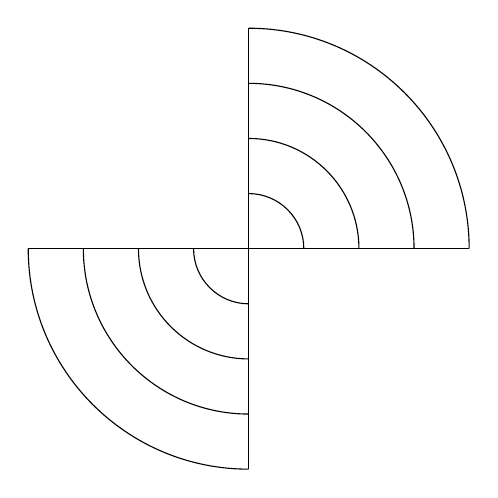
\begin{tikzpicture}[scale=0.7]
      % Draw the x and y axes
      \draw (-4,0) -- (4,0);
      \draw (0,-4) -- (0,4);
      
      \draw (1,0) arc (0:90:1);
      \draw (-1,0) arc (180:270:1);
      \draw (2,0) arc (0:90:2);
      \draw (-2,0) arc (180:270:2);
      \draw (3,0) arc (0:90:3);
      \draw (-3,0) arc (180:270:3);
      \draw (4,0) arc (0:90:4);
      \draw (-4,0) arc (180:270:4);
    \end{tikzpicture}
    \caption{Now note that $Y_1$ and $Y_2$ are both positive, and since $X_1$ and $X_2$ are both dependent on the same value of $W$, it is either $X_1$ and $X_2$ are both positive or both negative. So, the joint distribution of $X_1, X_2$ will be on only the 1st and 3rd quadrant with no mass on the 2nd and 4th. }
    \label{fig:not_multi_gaussian}
  \end{figure}
  \end{example}

\subsection{Multivariate Gaussians}

  There are three equivalent definitions of multivariate Gaussians of $n$-variables. 

  \begin{definition}[Multivariate Gaussian]
  Let us have a vector-valued random variable $\mathbf{X} = (X_1 \ldots X_n)^T \sim \mathcal{N}(\boldsymbol{\mu}, \boldsymbol{\Sigma})$. 
  \begin{enumerate}
      \item $\mathbf{X}$ is a \textbf{multivariate Gaussian distribution} with mean $\boldsymbol{\mu} \in \mathbb{R}^n$ and symmetric, positive-definite covariance matrix $\boldsymbol{\Sigma} \in \mathbb{R}^{n \times n}$ if its probability density function is
      \[f_X (x) = \frac{1}{(2\pi)^{n/2} \mathrm{det}(\boldsymbol{\Sigma})^{1/2}} \exp\bigg( -\frac{1}{2} (x-\boldsymbol{\mu})^T \boldsymbol{\Sigma}^{-1} (x - \boldsymbol{\mu})\bigg)\]
      The covariance matrix $\boldsymbol{\Sigma}$ is the $n \times n$ matrix whose $(i, j)$th entry is $\Cov(X_i, X_j)$. That is, for any random vector $\mathbf{X}$ with mean $\boldsymbol{\mu}$, its covariance matrix 
      \[\boldsymbol{\Sigma} = \mathbb{E}\big[ (\mathbf{X} - \boldsymbol{\mu}) (\mathbf{X} - \boldsymbol{\mu})^T \big] = \mathbb{E}[\mathbf{X} \mathbf{X}^T] - \boldsymbol{\mu} \boldsymbol{\mu}^T\]
      is positive definite and symmetric, which implies by the spectral theorem we can break it down into $n$ orthogonal eigenspaces of positive eigenvalues. 

      \item $X$ is a multivariate Gaussian distribution if it can be expressed as 
      \[\mathbf{X} = \mathbf{D} \mathbf{w} + \boldsymbol{\mu}\]
      where $\mathbf{w}$ is a vector of independent $\mathcal{N}(0, 1)$ Gaussians, $\boldsymbol{\mu} \in \mathbb{R}^n$, and $\mathbf{D} \in \mathbb{R}^{n \times n}$. The mean of $\mathbf{X}$ is $\boldsymbol{\mu}$ and its covariance is $\boldsymbol{\Sigma} = \mathbf{D} \mathbf{D}^T$; $\mathbf{D}$ is called the \textbf{standard deviation matrix}. When modeling high-dimensional Gaussians, this way is most computationally feasible. 

      \item $X$ is a multivariate Gaussian distribution if for every $\mathbf{a} \in \mathbb{R}^n$, $\mathbf{a}^T \mathbf{x}$ is a Gaussian RV. This means that if we take $\mathbf{a} = \mathbf{0}$, then the entire $\mathbf{X}$ is constantly $0$, which we will take to be the degenerate Gaussian with mean, variance $0$. 
  \end{enumerate}
  The $n$ semi-axes of the $(n-1)$-dimensional isocontour ellipsoid formed by an $n$-dimensional Gaussian distribution are precisely the normalized eigenvectors of $\boldsymbol{\Sigma}$ multiplied by their eigenvalues. 
  \end{definition}


  If we let $\boldsymbol{\Sigma} = \mathbf{I}$, then this means that all the $X_i$'s are pairwise uncorrelated since $\Sigma_{ij} = \Cov (X_i, X_j) = 0$. In general, this does not mean that the $X_i$'s are independent, but for joint Gaussians, this also implies independence! 

  \begin{theorem}
  Given multivariate Gaussian $\mathbf{X} = (X_1 \ldots X_n)^T \sim \mathcal{N}(\boldsymbol{\mu}, \boldsymbol{\Sigma})$, the $X_i$'s are pairwise independent if and only if they are uncorrelated. 
  \end{theorem}
  \begin{proof}
  We can expand the PDF of $\mathbf{X}$ as 
  \begin{align*}
      f_X (x) & = \frac{1}{(2 \pi)^{n/2}} \exp \bigg( -\frac{1}{2} (x - \mu)^T (x - \mu) \bigg) \\
      & = \bigg(\frac{1}{\sqrt{2\pi}} \bigg)^n \exp \bigg( \sum_{i=1}^n -\frac{1}{2} (x_i - \mu_i)^2 \bigg) \\
      & = \prod_{i=1}^n \frac{1}{\sqrt{2\pi}} \exp \bigg( -\frac{1}{2} (x_i - \mu_i)^2 \bigg)
  \end{align*}
  which is the product of $n$ single-variable Gaussians $X_i$. Therefore this means that independence and uncorrelation are equivalent! 
  \end{proof}

  Therefore, if the nondiagonal entries of the covariance matrix are all $0$, then we know that the variables are all uncorrelated and therefore independent. 

\section*{To Do: Functions of Random Variables}

  In many applications, it happens that we are interested not in the value of the random variable $X$, but a function of it. That is, given a probability space $(\Omega, \mathcal{F}, \mathbb{P})$, let us have a random variable $X: \Omega \rightarrow \mathbb{R}$. We can then define another function $f: \mathbb{R} \rightarrow \mathbb{R}$ and consider the potential random variable $f \circ X : \Omega \rightarrow \mathbb{R}$. We say potential because we don't know yet whether $f \circ X$ is measurable (i.e. the preimage of every Borel set in $\mathbb{R}$ is in $\mathcal{F}$). This condition suffices if $f$ itself is a measurable function, i.e. for every Borel set $B \in \mathcal{R}$, its preimage $f^{-1} (B)$ is Borel in $\mathbb{R}$, and by measurablility of $X$, its preimage under $X$ is $\mathcal{F}$-measurable, making $f \circ X$ a viable random variable. With this new random variable $f \circ X$, we would now like to answer the question: What is the probability law $\mathbb{P}_{f \circ X}$ of $\mathbb{R}$? 

  This also works for joint random variables, which we will learn later. Given a joint random variable $(X_1, X_2, \ldots X_n): \Omega \rightarrow \mathbb{R}^n$, we can define a measurable function $f: \mathbb{R}^n \longrightarrow \mathbb{R}$ and define the scalar random variable $f \circ (X_1, \ldots X_n)$ on $\Omega$. But again, we want to find what the CDF of this composition. 

\subsection{Convolutions and Sums of Random Variables}

  Now given two random variables $X, Y: \Omega \rightarrow \mathbb{R}$ that each push their own probability laws $\mathbb{P}_X, \mathbb{P}_Y$ onto $\mathbb{R}$, their sum $Z = X + Y$ is also a random variable that pushes its own probability law $\mathbb{P}_Z$. We must actually prove that $Z$ is a random variable, which we can do by proving that the preimage of every $(-\infty, x]$ is $\mathcal{F}$-measurable. Equivalently (by complementation), we must prove that the preimage of every $(x, +\infty)$ (that is, all sets of form $\{ \omega \mid Z(\omega) > z\}$) is $\mathcal{F}$-measurable. Now we can write $z$ as the sum of two numbers $z = q + (z - q)$, where $q \in \mathbb{R}$, and say that 
  \begin{equation}
    \{ \omega \mid Z(\omega) > z\} = \bigcup_{q \in \mathbb{R}} \{ \omega \mid X (\omega) > q , \; Y(\omega) > z - q\}
  \end{equation}
  But using the fact that $\mathbb{Q}$ is dense in $\mathbb{R}$, we can turn this from an uncountable union to a countable union and say 
  \begin{align}
    \{ \omega \mid Z(\omega) > z\} & = \bigcup_{q \in \mathbb{Q}} \{ \omega \mid X (\omega) > q , \; Y(\omega) > z - q\} \\
    & = \bigcup_{q \in \mathbb{Q}} \big( \{\omega \mid X(\omega) > q\} \cap \{ \omega \mid Y(\omega) > z - q\} \big) 
  \end{align}
  and since I have a countable union of (an intersection of) these $\mathcal{F}$-measurable sets, $\{ \omega \mid Z(\omega) > z\}$ is $\mathcal{F}$-measurable, and we are done. This equation above even gives us a hint of how to compute the CDF of $Z$. 

  \begin{theorem}
    Given random variables $X_1, X_2, \ldots, X_n$ of probability space $(\Omega, \mathcal{F}, \mathbb{P})$, 
    \begin{enumerate}
      \item $X_1 + \ldots + X_n$ is a random variable.
      \item $X_1 \cdot \ldots \cdot X_n$ is a random variable. 
    \end{enumerate}
  \end{theorem}

  For simplicity, we will only consider jointly discrete or jointly continuous random variables. The probability law $\mathbb{P}_Z$ can be confusing to define, since given some Borel set $B \in \mathcal{R}$, we must now look at the preimage under the \textit{sum} $X + Y$. A simpler way to approach this is to consider the joint distribution $X, Y$ and look at its distribution, which we call the \textbf{convolution} of $X$ and $Y$. This is especially simple to consider for discrete random variables. 

  \begin{definition}[Sums of Discrete Random Variables]
    Take two discrete random variables $X, Y$ with their joint PMF $p_{X, Y} (x, y)$ and their sum $Z = X + Y$. We can see that the PMF of $Z$ is 
    \begin{equation}
      p_Z (z) = \sum_{(x, y) \,:\, x + y = z} p_{X, Y} (x, y) = \sum_{x \in \mathcal{X}} p_{X, Y} (x, z - x)
    \end{equation}
    which by abuse of notation, we denote
    \begin{equation}
      \mathbb{P}(Z = z) = \sum_{x \in \mathcal{X}} \mathbb{P}(X = x, Y = z - x)
    \end{equation}
    The CDF is very simple, since we just have to sum over all $(x, y)$ such that their sum is less than $z$: 
    \begin{equation}
      F_Z (z) = \sum_{(x, y) \,:\, x + y \leq z} p_{X, Y} (x, y)
    \end{equation}
    which by abuse of notation, we write 
    \begin{equation}
      \mathbb{P}(Z \leq z) = \sum_{(x, y) \,:\, x + y \leq z} \mathbb{P}(X = x, Y = y)
    \end{equation}
    If $X$ and $Y$ are independent, then their joint distribution is the product of their singular distributions, and so we have 
    \begin{equation}
      p_Z (z) = \sum_x p_X (x) \, p_Y (z - x) \coloneqq p_X \ast p_Y
    \end{equation}
    where $p_Z = p_X \ast p_Y$ is called the convolution of $p_X$ and $p_Y$. By abuse of notation, 
    \begin{equation}
      \mathbb{P}(Z = z) = \sum_{x \in \mathcal{X}} \mathbb{P}(X = x) \, \mathbb{P}(Y = z - x)
    \end{equation}
  \end{definition}

  \begin{example}[Sums of Poisson RVs]
    Let $X_1$ and $X_2$ be independent Poisson random variables with parameters $\lambda_1, \lambda_2 > 0$, and let $Z = X_1 + X_2$. The PMF of each $X_i$ is 
    \begin{equation}
      p_{X_i} (k) = \frac{e^{-\lambda_i} \lambda_i^k}{k!} \text{ for } k \in \mathbb{Z}
    \end{equation}
    and taking the convolution gives the PMF of $Z$: 
    \begin{align*}
      p_Z (z) & = (p_{X_1} \ast p_{X_2}) (z) \\
      & = \sum_{k=-\infty}^{+\infty} \frac{e^{-\lambda_1} \lambda_1^k}{k!} \cdot \frac{e^{-\lambda_2} \lambda_2^{z - k}}{(z - k)!} \\
      & = \sum_{k=0}^{z} \frac{e^{-\lambda_1} \lambda_1^k}{k!} \cdot \frac{e^{-\lambda_2} \lambda_2^{z - k}}{(z - k)!} \\ 
      & = \frac{e^{-(\lambda_1 + \lambda_2)}}{z!} \sum_{k=0}^z \binom{z}{k} \lambda_1^k \lambda_2^{z - k} \\
      & = \frac{e^{-(\lambda_1 + \lambda_2)} (\lambda_1 + \lambda_2)^z}{z!} 
    \end{align*}
    for $z \in \mathbb{N}_0$, which is the PMF of another Poisson. So, $Z \sim \mathrm{Poisson}(\lambda_1 + \lambda_2)$. 
  \end{example}

  This has a nice visualization, since the joint distribution of $X$ and $Y$ over $\mathbb{R}^2$ is being "summed up/integrated" over the diagonals of $\mathbb{R}^2$, i.e. the lines where $x + y = z$ for some $z$, sort of like marginalizing over these diagonals. This creates a new "diagonally marginal distribution" $Z$. 

  \begin{definition}[Sums of Continuous Random Variables]
    Take two continuous random variables $X, Y$ with their joint PDF $f_{X, Y} (x, y)$ and their sum $Z = X + Y$. To calculate the CDF, we must basically integrate the joint PDF over the borel set $\{(x, y) \in \mathbb{R}^2 \mid x + y \leq z\}$. 
    \begin{align*}
      \mathbb{P}(Z \leq z) = F_Z (z) & = \int_{(x, y) \,:\, x + y \leq z} f_{X, Y} (x, y) \,dy\,dx \\
      & = \int_{-\infty}^{+\infty} \int_{-\infty}^{z - x} f(x, y) \,dy \,dx
    \end{align*}
    We can see that the PDF of $Z$ is 
    \begin{equation}
      f_{Z} (z) = \int_{\mathbb{R}} f_{X, Y} (x, z - x) \, dx
    \end{equation}
    If $X$ and $Y$ are independent, then 
    \begin{equation}
      f_{Z} (z) = \int_{\mathbb{R}} f_{X} (x) \, f_Y (z - x) \,dx \coloneqq f_X \ast f_Y
    \end{equation}
    where $f_Z = f_X \ast f_Y$ is the convolution of $f_X$ and $f_Y$. 
  \end{definition}

  \begin{definition}[Convolution]
    Given two functions $f, g: \mathbb{R} \longrightarrow \mathbb{R}$, the \textbf{convolution} of $f$ and $g$ is a new function $f \ast g$ defined  
    \begin{equation}
      (f \ast g) (t) \coloneqq \int_\mathbb{R} f(t)\, g(t - \tau) \, d \tau
    \end{equation}
  \end{definition}

  Usually, when we take convolutions, it is not pretty and even for nice distributions like two Gaussians, convolving them is quite complicated. What we can do is transform them (using Laplace, Fourier, etc.) to make calculations easier and more elegant, which we will talk about later.  

  \begin{example}
    Let $X_1$ and $X_2$ be independent exponential with parameters $\lambda_1, \lambda_2$, with individual PDFs $f_{X_i} (x) = \lambda_i e^{-\lambda_i x}$ for $x \geq 0$. Let $Z = X_1 + X_2$. Then, 
    \begin{align*}
      f_Z (z) = (f_{X_1} \ast f_{X_2})(z) & = \int_{-\infty}^\infty \lambda_1 e^{-\lambda_1 x} \, \lambda_2 e^{-\lambda_2 (z -x)} \, dx \\
      & = \int_{0}^z \lambda_1 e^{-\lambda_1 x} \, \lambda_2 e^{-\lambda_2 (z -x)} \, dx \\ 
      & = \lambda_1 \lambda_2 e^{-\lambda_2 z} \int_0^z e^{(\lambda_2 - \lambda_1) x}\,dx \\
      & = \begin{cases} \frac{\lambda_1 \lambda_2}{\lambda_2 - \lambda_1} \big( e^{-\lambda_1 z} - e^{-\lambda-2 z} \big) & \text{ if } \lambda_1 \neq \lambda_2 \\
      \lambda^2 z e^{-\lambda z} & \text{ if } \lambda_1 = \lambda_2 = \lambda \end{cases} 
    \end{align*}
    The distribution for when $\mu_1 = \mu_2$ is called the Erlang distribution, which has many applications, but the other case is an ugly form and not studied very well. 
  \end{example}

  \begin{theorem}[Sums of Discrete Variables]
    Assume that $X$ and $Y$ are independent. 
    \begin{enumerate}
      \item $X \sim$ Binomial$(n, p)$, $Y \sim$ Binomial$(m, p)$ $\implies X + Y \sim$ Binomial$(n + m, p)$. 
      \item $X \sim$ Poisson$(\lambda)$, $Y \sim$ Poisson$(\gamma)$ $\implies X + Y \sim$ Poisson$(\lambda + \gamma)$. 
      \item If $X_1, ..., X_n$ are Geometric$(p)$, then $X_1 + ... + X_n$ is NB$(n, p)$. 
    \end{enumerate}
  \end{theorem}

  \begin{theorem}[Sums of Densities]
    Assume that $X$ and $Y$ are independent. 
    \begin{enumerate}
      \item $X \sim$ Normal$(\mu_1, \sigma_1^2)$, $Y \sim$ Normal$(\mu_2, \sigma_2^2)$ $\implies X + Y \sim$ Normal $(\mu_1 + \mu_2, \sigma_1^2 + \sigma_2^2)$. 
      \item If $X_1, X_2, ..., X_n$ are Exponential$(\lambda)$, then $X_1 + ... + X_n \sim$ Gamma$(n, \lambda)$.
      \item $X \sim$ Gamma$(n, \lambda)$, $Y \sim$ Gamma$(m, \lambda)$ $\implies X + Y \sim$ Gamma$(n + m, \lambda)$. 
      \item $X \sim$ Gamma $(n, \lambda)$, $Y \sim$ Exponential $(\lambda)$ $\implies X + Y \sim$ Gamma$(n+1, \lambda)$. 
    \end{enumerate}
  \end{theorem}

\subsection{Order Statistics}

  Let $X_1, X_2, \ldots, X_n$ be random variables of $(\Omega, \mathcal{F}, \mathbb{P})$ with joint CDF $F_{X_1 \ldots X_n} (x_1, \ldots, x_n)$. Let $Y_n = \min (X_1, \ldots, X_n)$ and $Z_n = \max(X_1, \ldots, X_n)$. Note that $Y_n$ and $Z_n$ are also functions of $\Omega$ to $\mathbb{R}$. To prove that they are random variables, we just have to prove that $\min$ and $\max$ are measurable functions from $\mathbb{R}^n$ to $\mathbb{R}$, which we can do by proving that the preimage of all semi-infinite interval $(-\infty, x]$ are Borel in $\mathbb{R}^n$. 
  \begin{enumerate}
    \item The preimage of $(-\infty, x]$ under $\max$ is just the set of all $n$-vectors whose max is less than $x$, which is just the semi-infinite cuboid $(-\infty, x]^n \subset \mathbb{R}^n$, which is Borel in $\mathbb{R}^n$. 
    \item The preimage of $(-\infty, x]$ under $\min$ is the set of all $n$-vectors whose min is less than $x$, i.e. at least one element must be less than $x$. But this is just the complement of all vectors that have elements all greater than $x$, which is $\mathbb{R}^n \setminus (x, +\infty)^n \subset \mathbb{R}^n$, which is Borel in $\mathbb{R}^n$. 
  \end{enumerate}
  Now we must determine the CDF of $Y_n$ and $Z_n$. 
  \begin{enumerate}
    \item We have 
    \begin{align*}
      F_{Z_n} (z) & = \mathbb{P}(\{ \omega \mid Z_n (\omega) \leq z \}) \\
      & = \mathbb{P}(\{ \omega \mid X_1 (\omega) \leq z, \ldots, X_n (\omega) \leq z\}) \\
      & = F_{X_1 \ldots X_n} (z, \ldots, z)
    \end{align*}
    where the last equality is describes simply the joint CDF of the joint distribution $(X_1, \ldots, X_n)$. If we assume independence of $X_i$'s, it simplifies out to 
    \begin{equation}
      \prod_{i} F_{X_i} (z)
    \end{equation}
    and if iid, then we have $[F_{X} (z) ]^n$, where $X$ is the common distribution. 
    \item For $Y_n$, we work with complements again and have 
    \begin{align*}
      F_{Y_n} (y) & = \mathbb{P}(\{ \omega \mid Y_n (\omega) \leq y \}) \\ 
      & = 1 - \mathbb{P}(\{ \omega \mid Y_n (\omega) > y \}) \\
      & = 1 - \mathbb{P}(\{ \omega \mid X_1 (\omega) > y, \ldots X_n (\omega) > y \}) \\
    \end{align*}
    where $\mathbb{P}(\{ \omega \mid X_1 (\omega) > y, \ldots X_n > y \})$ can be calculated from the joint distribution. If we assume independence of $X_i$, it simplifies out to 
    \begin{equation}
      1 - \prod_{i} \mathbb{P}(\{\omega \mid X_i(\omega) > y \}) = 1 - \prod_{i} \big( 1 - F_{X_i} (y) \big)
    \end{equation}
    and if iid, then we have $1 - [1 - F_{X} (y)]^n$. 
  \end{enumerate}

  \begin{example}[Uniforms]
    Let $X_1, X_2$ be iid distributed as $\mathrm{Uniform}[0, 1]$, and let $Z = \max(X_1, X_2)$ with $Y = \min(X_1, X_2)$, i.e. $Z$ is the greater of the two and $Y$ is the lesser. We would expect the PDF of $Z$ to have more mass towards $1$ and the PDF of $Y$ to have more mass towards $0$. Our common CDF is 
    \begin{equation}
      F_{X} (x) = \begin{cases} 0 & \text{ if } x < 0 \\
      x & \text{ if } 0 \leq x \leq 1 \\
      1 & \text{ if } 1 < x \end{cases}
    \end{equation}
    Let's calculate the CDF of $Z$. 
    \begin{align*}
      F_{Z} (z) & = \mathbb{P}(\{\omega \mid Z(\omega) \leq z\}) \\
      & = \mathbb{P}(\{ \omega \mid X_1 (\omega) \leq z, X_2 (\omega) \leq z\}) \\
      & = F_{X_1, X_2} (z, z) \\
      & = [F_{X} (z)]^2 = \begin{cases} 0 & \text{ if } x < 0 \\
      x^2 & \text{ if } x \in [0, 1] \\
      1 & \text{ if } 1 < x \end{cases}
    \end{align*}
    This CDF is differentiable everywhere except the two points $0$ and $1$, so we can get the PDF to be $f_Z (z) = 2 z$ for $z \in (0, 1)$ and $0$ otherwise. For the values of $f_Z$ at $0$ and $1$, we can fill it in with anything we want (since the measure of these sets are $0$), so we will just defined $f_Z (0) = 0$ and $f_Z(1) = 2$, getting 
    \begin{equation}
      f_Z (z) = \begin{cases} 2 z & \text{ if } z \in [0, 1] \\
      0 & \text{ if else} \end{cases}
    \end{equation}
    Let's calculate the CDF of $Y$. 
    \begin{align*}
      F_{Y} (y) & = \mathbb{P}(\{ \omega \mid Y(\omega) \leq y\}) \\
      & = 1 - \mathbb{P}(\{ \omega \mid Y(\omega) > y\}) \\
      & = 1 - \mathbb{P}(\{\omega \mid X_1 (\omega) > y, X_2 (\omega) > y \}) \\
      & = 1 - \mathbb{P}(\{\omega \mid X_1 (\omega) > y\}) \, \mathbb{P}(\{ X_2 (\omega) > y \}) \\ 
      & = 1 - [1 - F_X (y)]^2 = \begin{cases} 0 & \text{ if } y < 0 \\
      1 - (1 - y)^2 & \text{ if } y \in [0, 1] \\
      1 & \text{ if } y > 1 \end{cases} 
    \end{align*}
    and differentiating it (with setting any values of the PDF at the nondifferentiable points $0$ and $1$) gives 
    \begin{equation}
      f_Y (y) = \begin{cases} 2 - 2y & \text{ if } y \in [0, 1] \\
      0 & \text{ if else} \end{cases}
    \end{equation}
  \end{example}

  \begin{example}[Exponentials]
    Let $X_1, X_2, \ldots, X_n$ be independent exponential random variables with parameters $\lambda_1, \ldots, \lambda_n$, respectively (not identical!). Then, for each $X_i$, its CDF is 
    \begin{equation}
      F_{X_i} (x) = 1 - e^{-\lambda_i x} \text{ for } x \geq 0
    \end{equation}
    and let $Y = \min(X_1, \ldots, X_n)$. Then, we have 
    \begin{align*}
      F_Y (y) & = 1 - \prod_{i=1}^n [ 1 - F_{X_i} (y)] \\
      & = 1 - \prod_{i=1}^n e^{-\lambda_i x} \\
      & = 1 - e^{- ( \sum_{i=1}^n \lambda_i ) x}
    \end{align*}
    which is the CDF of an exponential distribution. So, 
    \begin{equation}
      Y \sim \mathrm{Exponential}(\lambda_1 + \ldots + \lambda_n)
    \end{equation}
    This is nice, since the minimum of a bunch of exponentials is an exponential. However, this is not the case for the maximum. 
  \end{example}

  This has nice practical applications. For example, recall the memoryless property of the exponential, which nicely models radioactive decay. If we have $n$ elements each decaying at some $\mathrm{Exponential}(\lambda_i)$ rate, then we can model the time at which the first alpha particle will emit amongst all $n$ elements will also be an exponential. These processes where the inter-emission times are exponentials are called Poisson process, which we will discuss later. 

  \begin{definition}[Order Statistic]
    Let $X_1, X_2, ..., X_n$ be a finite collection of independent, identically distributed random variables. Suppose that they are continuously distributed with density $f$ and CDF $F$. Define the random variable $X_{(k)}$ to be the $k$th ranked value, called the \textbf{$k$th order statistic}. This means that 
    \begin{equation}
      X_{(1)} = \min\{X_1, X_2, ..., X_n\}, \;\; X_{(n)} = \max\{X_1, X_2, ..., X_n\}
    \end{equation}
    and in general, for any $k \in \{1, 2, ..., n\}$, 
    \begin{equation}
      X_{(k)} = X_j \text{ if } \sum_{l=1}^n \mathbb{I}_{X_l < X_j} = k - 1
    \end{equation}
    which means that exactly $k-1$ of the values of $X_l$ are less than $X_j$. Since $F$ is continuous, 
    \begin{equation}
      X_{(1)} < X_{(2)} < ... < X_{(n)}
    \end{equation}
    holds with probability $1$. This leads us to define the random variable $X_{(k)}$ representing the $k$th order statistic.
    \begin{equation}
      f_{(k)} (y) = \begin{cases} 
      n \, \binom{n-1}{k-1} y^{k-1} (1-y)^{n-k} & y \in (0, 1) \\
      0 & y \not\in (0,1)
      \end{cases}
    \end{equation}
    That is, $X_{(k)}$ has the Beta$(k, n-k_1)$ distribution. 
  \end{definition}

\subsection{Poisson Arrival Process}

  A \textbf{Poisson Arrival Process} with rate $\lambda > 0$ on the interval $[0, \infty)$ is a model for the occurence of some events which may have at any time. We can interpret the process as a collection of random points in $[0, \infty)$ which are the times at which the arrivals occur. 
  \begin{enumerate}
    \item \textit{Interpretation 1}. Set $T_0 = 0$. The arrival times are random variables $0 < T_1 < T_2 < T_3 < ...$ such that the inter-arrival waiting times
    \begin{equation}
      W_k = T_k - T_{k-1}, \;\;\; k \geq 0
    \end{equation}
    have the property that $\{W_k\}_{k=1}^\infty$ are independent Exp$(\lambda)$ random variables. 

    \item \textit{Interpretation 2}. For any interval $I \subset [0, \infty)$, let 
    \begin{equation}
      N_I \equiv \text{ number of arrivals that occur in interval } I
    \end{equation}
    Then, $N_I \sim$ Poisson$(\lambda |I|)$, and for any collection of disjoint intervals $I_1, I_2, ..., I_n$, the random variables 
    \begin{equation}
      \{N_{I_k}\}_{k=1}^n
    \end{equation}
  are independent. 
  \end{enumerate}

  \begin{theorem}
    These two interpretations of the arrival process are equivalent. 
  \end{theorem}
  \begin{proof}
    In the 2nd interpretation, the statement $N_I \sim$ Poisson$(\lambda |I|)$ means that 
    \begin{equation}
      \mathbb{P}(N_I = m) = e^{-\lambda |I|} \frac{(\lambda |I|)^m}{m!}, \;\;\; m = 0, 1, 2, 3, ...
    \end{equation}
    where $|I|$ is the length of interval $I$. From the first perspective, notice that 
    \begin{equation}
      T_k = W_1 + W_2 + ... + W_k
    \end{equation}
    so that the $k$th arrival time $T_k$ is a sum of $k$ independent Exp$(\lambda)$ random variables. Thus, 
    \begin{equation}
      T_k \sim \text{Gamma}(k, \lambda)
    \end{equation}
    and therefore has density
    \begin{equation}
    \lambda e^{-\lambda t} \frac{(\lambda t)^{k-1}}{(k-1)!}, \;\;\; t>0
    \end{equation}
    Note that the arrival times $T_i$ are not independent of each other, but the wait times $W_i$ are indeed independent. 
  \end{proof}

  We can slightly modify this to create a Poisson arrival process over some finite time horizon $[0, L]$. Again, you can do this two ways: 
  \begin{enumerate}
    \item Starting with independent Exp$(\lambda)$ random variables $W_1, W_2, ...$, we define
    \begin{equation}
      T_k = \sum_{i=1}^k W_i
    \end{equation}
    Once you have $T_k > L$, stop. 
    \item We let $N \sim$ Poisson$(\lambda L)$, since we are only working in finite interval $L$. Given $N = n$, let $U_1, U_2, ..., U_n \sim$ Uniform$([0, L])$. These define the arrival times, and let us order them to get
    \begin{equation}
      T_k = U_{(k)}, \;\; k = 1, 2, ..., N
    \end{equation}
    where $U_{(k)}$ is the $k$th ordered point, with $T_1 = \min(U_1, ..., U_N)$. 
  \end{enumerate}

  \begin{lemma}[Memoryless Property]
    The Exp$(\lambda)$ distribution has the property that for all $t, s \geq 0$, 
    \begin{equation}
      \mathbb{P}(W > t + s \; | \; W > t) = \mathbb{P}(W > s)
    \end{equation}
    which is called the \textit{memoryless property}. We can interpret this in the following way. Let $W$ be the time you have to wait for the first arrival. Given that you already waited $t$ units of time, the probability that you have the wait $s$ additional units of time is just the probability that you wait at least $s$ from the beginning. That is, knowing that $t$ units of time have elapsed does not affect the distribution of the remaining waiting time. 
  \end{lemma}

  \begin{theorem}
    Let $W$ be a continuously distributed random variable. Then $W \sim$ Exp$(\lambda)$ for some $\lambda > 0$ if and only if $W$ satisfies the memoryless property. 
  \end{theorem}

\subsection{Sum of Random Number of Random Variables}

  Now we consider a random variable where the number of terms we are summing is a random variable. Let $\{X_i\}_i$ be a countable sequence of independent random variables with CDF $F_{X_i}$. Let $N$ be a positive integer-valued random variable with PMF $p_N(n) = \mathbb{P}(N = n)$. Assume that $N$ is independent of $X_i$'s. Now, consider the function 
  \begin{equation}
    S_N \coloneqq \sum_{i=1}^N X_i
  \end{equation}
  To interpret this, consider the sample space $\Omega$. We have all $X_i$'s and $N$ defined on the same $\Omega$. Once $\omega \in \Omega$ realizes, the $\{X_i\}$'s will realize as a sequence of numbers, and $N$ will realize as a positive integer. We simply sum them up according to the rule $S_N$, and by this definition, $S_N$ is a real-valued function on $\Omega$. We first have to prove that $S_N$ is a random variable (since we only know that a \textit{fixed} sum of random variables is a random variable), and then we must find the CDF of $S_N$ $\mathbb{P}(S_N \leq x)$. 

  First, note that the realization of $N$ partitions the sample space as 
  \begin{equation}
    \Omega = \bigsqcup_{n = 1}^\infty \{\omega \mid N(\omega) = n\}
  \end{equation}
  Once I have this partition, I can invoke the partition rule and write 
  \begin{align*}
    \mathbb{P}(S_N \leq x) & = \sum_{k=1}^\infty \mathbb{P}(S_N \leq x \mid N = k) \, \mathbb{P}(N = k) \\
    & = \sum_{k=1}^\infty \mathbb{P}(S_k \leq x \mid N = k) \, \mathbb{P}(N = k) & (\text{conditioned on } N = k) \\
    & = \sum_{k=1}^\infty \mathbb{P}(S_k \leq x) \, \mathbb{P}(N = k) & (N \text{ is indep. of } X_i \text{s})
  \end{align*}
  where $\mathbb{P}(N = k)$ is known since we know the PMF of $N$, and the CDFs $\mathbb{P}(S_k \leq x)$ can be computed by computing the deterministic sums and computing their CDF. 

  \begin{example}
    Let $X_i$'s be iid $\mathrm{Exponential}(\lambda)$, and $N \sim \mathrm{Geometric}(p)$. We know that the deterministic sum of iid exponentials gives an Erlang. So, $S_N = \sum_{i=1}^N X_i$, and its CDF is 
    \begin{equation}
      \mathbb{P}(S_N \leq x) = \sum_{k=1}^\infty \mathbb{P}(S_k \leq x) \, \mathbb{P}(N = k)
    \end{equation}
    where $\mathbb{P}(N = k) = (1 - p)^{k - 1} p$. The PDF of the Erlang is 
    \begin{equation}
      p_{S_k} (x) = \frac{\lambda^n x^{n-1}}{(n - 1)!} e^{-\lambda x}
    \end{equation}
    and doing the brute force calculations gives a clean $S_N \sim \mathrm{Exponential}(\lambda p)$. 
  \end{example}

\subsection{General Transformations of Random Variables}

  Now we will look at more general transformations that are not just minimum, maximum, deterministic sums, or random sums. Let us have a probability space $(\Omega, \mathcal{F}, \mathbb{P})$, a random variable $X: \Omega \rightarrow \mathbb{R}$, and a measurable function $f: \mathbb{R} \rightarrow \mathbb{R}$. Now given that we know the CDF (and therefore distribution) of $X$, we want to find the CDF of random variable $Y = f(X) = f \circ X$ (which we have established as a random variable already due to measurability of $f$): $F_Y (y) = \mathbb{P}(Y \leq y)$, which is just $\mathbb{P}_Y ((-\infty, y])$ (where $\mathbb{P}_Y$ is the probability law on $Y$). But rather than trying to take the preimage of the entire composite random variable $Y$ and calculating $\mathbb{P}\big( Y^{-1}((-\infty, y]) \big)$ under the probability on $\mathcal{F}$, let's just take the preimage one step at a time. Note that $f^{-1} \big( (-\infty, y] \big) = \{x \in \mathbb{R} \mid f(x) \leq y\}$. We can then write the CDF of $Y$ in terms of the probability law of $X$: 
  \begin{align*}
    F_Y (y) & = \mathbb{P}_X \big( f^{-1} ((-\infty, y]) \big) \\
    & = \mathbb{P}_X \big( \{x \in \mathbb{R} \mid f(x) \leq y\} \big) \\
    & = \mathbb{P} \big( X^{-1} \circ f^{-1} ((-\infty, y]) \big) 
  \end{align*}
  Depending on how complicated $f$ is, this may be easy or not, but conceptually, this is no problem. But theoretically, this is as far as we can go. Let's move onto some examples. We start with a practical way to generate a Gaussian distribution, which is how most modern software computes. 

  \begin{example}[Box-Muller Transform]
    Given that you have a uniform random number generator in $[0, 1]$, you can generate a normal $N(0, 1)$ by transforming it using the inverse CDF of the normal. This is usually computationally heavy since the inverse CDF of the Gaussian requires expensive operations. An easier way is to use the \textbf{Box-Muller transform}, where you take two uniforms $u_1, u_2$ and transform it as 
    \begin{align*}
        x_1 & = \sqrt{-2 \ln(u_1)} \cos(2 \pi u_2) \\
        x_2 & = \sqrt{-2 \ln(u_1)} \sin(2 \pi u_2)
    \end{align*}
    Once you have $x \sim N(0, 1)$, you can use $\mu + \sigma x \sim N(\mu, \sigma^2)$. You can extend this to a $n$-dimensional normal distribution $\mathbf{x} \sim N(\mathbf{0}, \mathbf{I})$ and transform it to get $\boldsymbol{\mu} + \boldsymbol{\Sigma}^{1/2} \mathbf{x} \sim N(\boldsymbol{\mu}, \boldsymbol{\Sigma})$. 
  \end{example}

  \begin{example}[Chi-Squared Distribution]
    Let $X \sim \mathcal{N}(0, 1)$ and $Y = f(X) = X^2$. Note that $X$ takes values in $(-\infty, +\infty)$ and $Y$ in $[0, +\infty)$. Then, we can write 
    \begin{align*}
      F_Y (y) & = \mathbb{P}(Y \leq y) \\ 
      & = \mathbb{P}_Y ( (-\infty, y]) \\
      & = \mathbb{P}_Y (  [0, y]) & (\text{range of } Y) \\
      & = \mathbb{P}_X ( f^{-1} ([0, y]) ) & (\text{work in prob. law of } X) \\
      & = \mathbb{P}_X ( [-\sqrt{y}, \sqrt{y}] ) \\
      & = \int_{-\sqrt{y}}^{\sqrt{y}} f_X (x) \,dx 
    \end{align*}
    Rewriting this in our abuse of notation notation, we have 
    \begin{align*}
      F_Y (y) & = \mathbb{P}(Y \leq y) \\
      & = \mathbb{P}(X^2 \leq y) \\
      & = \mathbb{P}( -\sqrt{y} \leq X \leq \sqrt{y}) \\
      & = 2 \mathbb{P}(0 \leq X \leq \sqrt{y}) & (\text{Symmetry of Gaussian})\\
      & = \frac{2}{\sqrt{2} \pi} \int_0^{\sqrt{y}} e^{-x^2 / 2} \,dx 
    \end{align*}
    and this is clearly differentiable, since it is written like an integral. Doing so gives the PDF
    \begin{equation}
      f_Y (y) = \frac{1}{\sqrt{2 \pi y}} e^{-y/2} \text{ for } y \geq 0
    \end{equation}
    This describes the PDF of a \textbf{Chi-Squared} distribution. 
  \end{example}

  \begin{example}[Log-Normal Distribution]
    Let $X \sim \mathcal{N}(0, 1)$ and $Y = f(X) = e^X$. Note that the range of $f$ is $(0, +\infty)$. So, 
    \begin{align*}
      F_Y (y) & = \mathbb{P}(Y \leq y) \\
      & = \mathbb{P}_Y ((-\infty, y]) \\
      & = \mathbb{P}_Y ( (0, y]) \\ 
      & = \mathbb{P}_X ( f^{-1} ((0, y]) ) \\
      & = \mathbb{P}_X ( (-\infty, \ln{y}] ) \\
      & = \int_{-\infty}^{\ln{y}} f_X (x)\,dx 
    \end{align*}
    Rewriting this in our abuse of notation notation, we have 
    \begin{align*}
      F_Y (y) & = \mathbb{P}(e^X \leq y) \\
      & = \mathbb{P}(X \leq \ln(y)) \\ 
      & = \int_{-\infty}^{\ln(y)} \frac{1}{\sqrt{2} \pi} e^{-x^2/ 2} \,dx 
    \end{align*}
    We can differentiate this to get 
    \begin{equation}
      f_Y (y) = \frac{1}{y \sqrt{2 \pi}} e^{-\frac{(ln{y})^2}{2}} \text{ for } y \geq 0
    \end{equation}
    This describes the PDF of a \textbf{log-normal} distribution. 
  \end{example}

  We now show a more specific formula under more specific assumptions about the transformation. Suppose $X$ is a \textit{continuous} random variable with density $f_X$ and $g: \mathbb{R} \rightarrow \mathbb{R}$ a monotonic differentiable function. Then, the CDF of the random variable $Y = g(X)$ can be written in the probability law of $X$, which can then by written as an integral by invoking the Radon-Nikodym theorem: 
  \begin{align*}
    \mathbb{P}(Y \leq y) & = \mathbb{P}_X (f^{-1} ((-\infty, y]) \\
    & = \int_{x \,:\, g(x) \leq y} f_X (x) \,dx
  \end{align*}
  Note that we can now talk about the actual inverse $g^{-1}$ since differentaible and monotonic implies invertibility. 
  \begin{enumerate}
    \item Assuming $g$ is monotonically increasing, we can use the change of variables $x = g^{-1} (t)$ and $g(x) = t \implies g^\prime (x) \,dx = dt$ to get the above integral as 
    \begin{equation}
      \int_{-\infty}^{g^{-1} (y)} f_X (x) \,dx = \int_{-\infty}^t \frac{f_X \big( g^{-1} (t) \big)}{g^\prime \big( g^{-1} (t)\big)} \,dt 
    \end{equation}
    but since this is simply the CDF of $Y$, the PDF must equal 
    \begin{equation}
      f_Y (y) = \frac{f_X (g^{-1} (y) )}{g^\prime (g^{-1} (t))}
    \end{equation}
    \item If $g$ is monotonically decreasing, we get 
    \begin{equation}
      f_Y (y) = \frac{f_X (g^{-1} (y) )}{- g^\prime (g^{-1} (t))}
    \end{equation}
  \end{enumerate}
  In general, we can consider both cases by putting an absolute value 
  \begin{equation}
    f_Y (y) = \frac{f_X (g^{-1} (y) )}{|g^\prime (g^{-1} (t))|}
  \end{equation}
  and $g^\prime (g^\prime (y))$ is the Jacobian, the same one that we use when we perform a change of variables in integration. 

  \begin{example}[Log-Normal Revisited]
    Given $X \sim \mathcal{N}(0, 1)$ and $Y = e^X$ (which is monotonically increasing), we can simply plug in the formula to get the PDF: 
    \begin{equation}
      f_Y (y) = \frac{f_X (g^{-1} (y) )}{|g^\prime (g^{-1} (t))|} = \frac{f_X (\ln{y}) }{ | e^{\ln{y}} |} = \frac{1}{\sqrt{2 \pi} y} e^{-(\ln{y})^2 / 2}
    \end{equation}
    for $y > 0$. This domain is important since $\ln{y}$ is only defined for $y > 0$. 
  \end{example}

  \begin{example}
    Given $X \sim \mathcal{N}(0, 1)$ and $Y = f(X) = X^2$, we cannot use the formula since $f$ is not monotonic on the range of $X$, which is $(-\infty, +\infty)$.  
  \end{example}

  \begin{example}
    Given $X \sim \mathrm{Exponential}(\lambda)$ and $Y = f(X) = X^2$, it may seem like the formula is not applicable here, but $f$ \textit{is} monotonic on the range of $X$, which is $[0, + \infty)$. 
  \end{example}

  However, there is much less chance of error by deriving using first principles, so I would recommend using it always rather than these formulas. 

  Let's do the $n$-dimensional version of this. Given random variables $X_1, X_2, \ldots, X_n$ iid random variables with joint density $f_{X_1 \ldots X_n} (x_1, \ldots, x_n)$, we define the transformation $g: \mathbb{R}^n \rightarrow \mathbb{R}^n$ as 
  \begin{equation}
    \begin{bmatrix} Y_1 \\ \vdots \\ Y_N \end{bmatrix} = \begin{bmatrix} g_1 (X_1) \\ \vdots \\ g_n (X_N) \end{bmatrix}
  \end{equation}
  Then, the PDF of $Y$ will be 
  \begin{align*}
    f_{Y_1 \ldots Y_n} (y_1, \ldots, y_n) & = f_{X_1 \ldots X_n} \big( \mathbf{g}^{-1} (\mathbf{y}) \big) \cdot | \mathbf{J}(\mathbf{y})| \\
    & = f_{X_1 \ldots X_n} \big( g_1^{-1}(y_1), \ldots, g_n^{-1} (y_n) \big) \cdot | \mathbf{J}(\mathbf{y})| \\
  \end{align*}
  where 
  \begin{equation}
    \mathbf{J}(y) = \mathrm{det}\begin{pmatrix} 
    \frac{\partial x_1}{\partial y_1} & \ldots & \frac{\partial x_n}{\partial y_1} \\
    \vdots & \ddots & \vdots \\ 
    \frac{\partial x_1}{\partial y_n} & \ldots & \frac{\partial x_n}{\partial y_n} \end{pmatrix}
  \end{equation}



